\section{Final testing and conclusions}\label{sec:conclusions}

Once we refined our model at the best could, we evaluated it against never seen data, by comparing the values predicted by the model, when the testing set is provided as input, against the true values of the annotations in the testing set. As already mentioned in section~\ref{sec:cross-validation}, once the final testing is done, we avoided going back to the model and make further tweaks, as this would have led to over-fitting.

For the final test we used the metrics of MSE and $R^2$-score (see section~\ref{sec:metrics}) and obtained the values reported in table~\ref{table:eval-metrics}. Despite several attempts and tests with different combinations of features, our results are not still optimal, in particular the $R^2$-score associated to the regressors of the two standard deviations. \todo[inline]{è una ripetizione della fine di evaluation, quel che conta è confrontare gli R2 di cross con R2 finali}

We also extracted scatter plots comparing the predictions of each regressor against the true values of the testing set. In  figure~\ref{fig:eval-scatter} is depicted the case of $\nu$-SVM, which turned out to be the best model fitting the data. In the best case scenario, these scatters should draw a 45° line. In our case, the scattering of ``valence std'' and ``arousal std'' clearly outline the bad $R^2$-scores obtained for these annotations. \todo{da finire}

The motivation of our results could be related to the composition of the dataset and the fact that we used only the part containing static annotations. A dynamic approach in which we consider values related to temporal windows and not to the total length of the music piece could have given different results. \todo{riscriverlo meglio forse}

\begin{table}
	\centering
	\todo[inline]{spostare tabella in dataset}
	\begin{tabular}{cccc}
		\toprule
		valence mean & valence std & arousal mean & arousal std \\
		\midrule
	    5.794 & 6.746 & 5.043 & 5.802 \\
		\bottomrule
	\end{tabular}
	\caption{Range (i.e. max-min) for each annotation after the standardization}
	\label{table:annot-ranges}
\end{table}

\begin{table}
	\centering
	\subcaptionbox{MSEs}{
		\begin{tabular}{lcccc}
			\toprule
			& valence mean & valence std & arousal mean & arousal std \\
			\midrule
			Ridge & 0.53 & 1.09 & 0.54 & 1.18 \\
			$\nu$-SVM & 0.58 & 1.00 & 0.49 & 1.09 \\
			K-neighbors & 0.62 & 1.00 & 0.61 & 1.08 \\
			\bottomrule
		\end{tabular}
	}
	\subcaptionbox{$R^2$-scores}{
		\begin{tabular}{lcccc}
			\toprule
			& valence mean & valence std & arousal mean & arousal std \\
			\midrule
			Ridge & 0.45 & -0.08 & 0.45 & -0.09 \\
			$\nu$-SVM & 0.40 & 0.01 & 0.50 & 0.00 \\
			K-neighbors & 0.35 & 0.01 & 0.39 & 0.00 \\
			\bottomrule
		\end{tabular}
	}
	\caption{Final evaluation metrics}
	\label{table:eval-metrics}
\end{table}

\begin{figure}
	\centering
	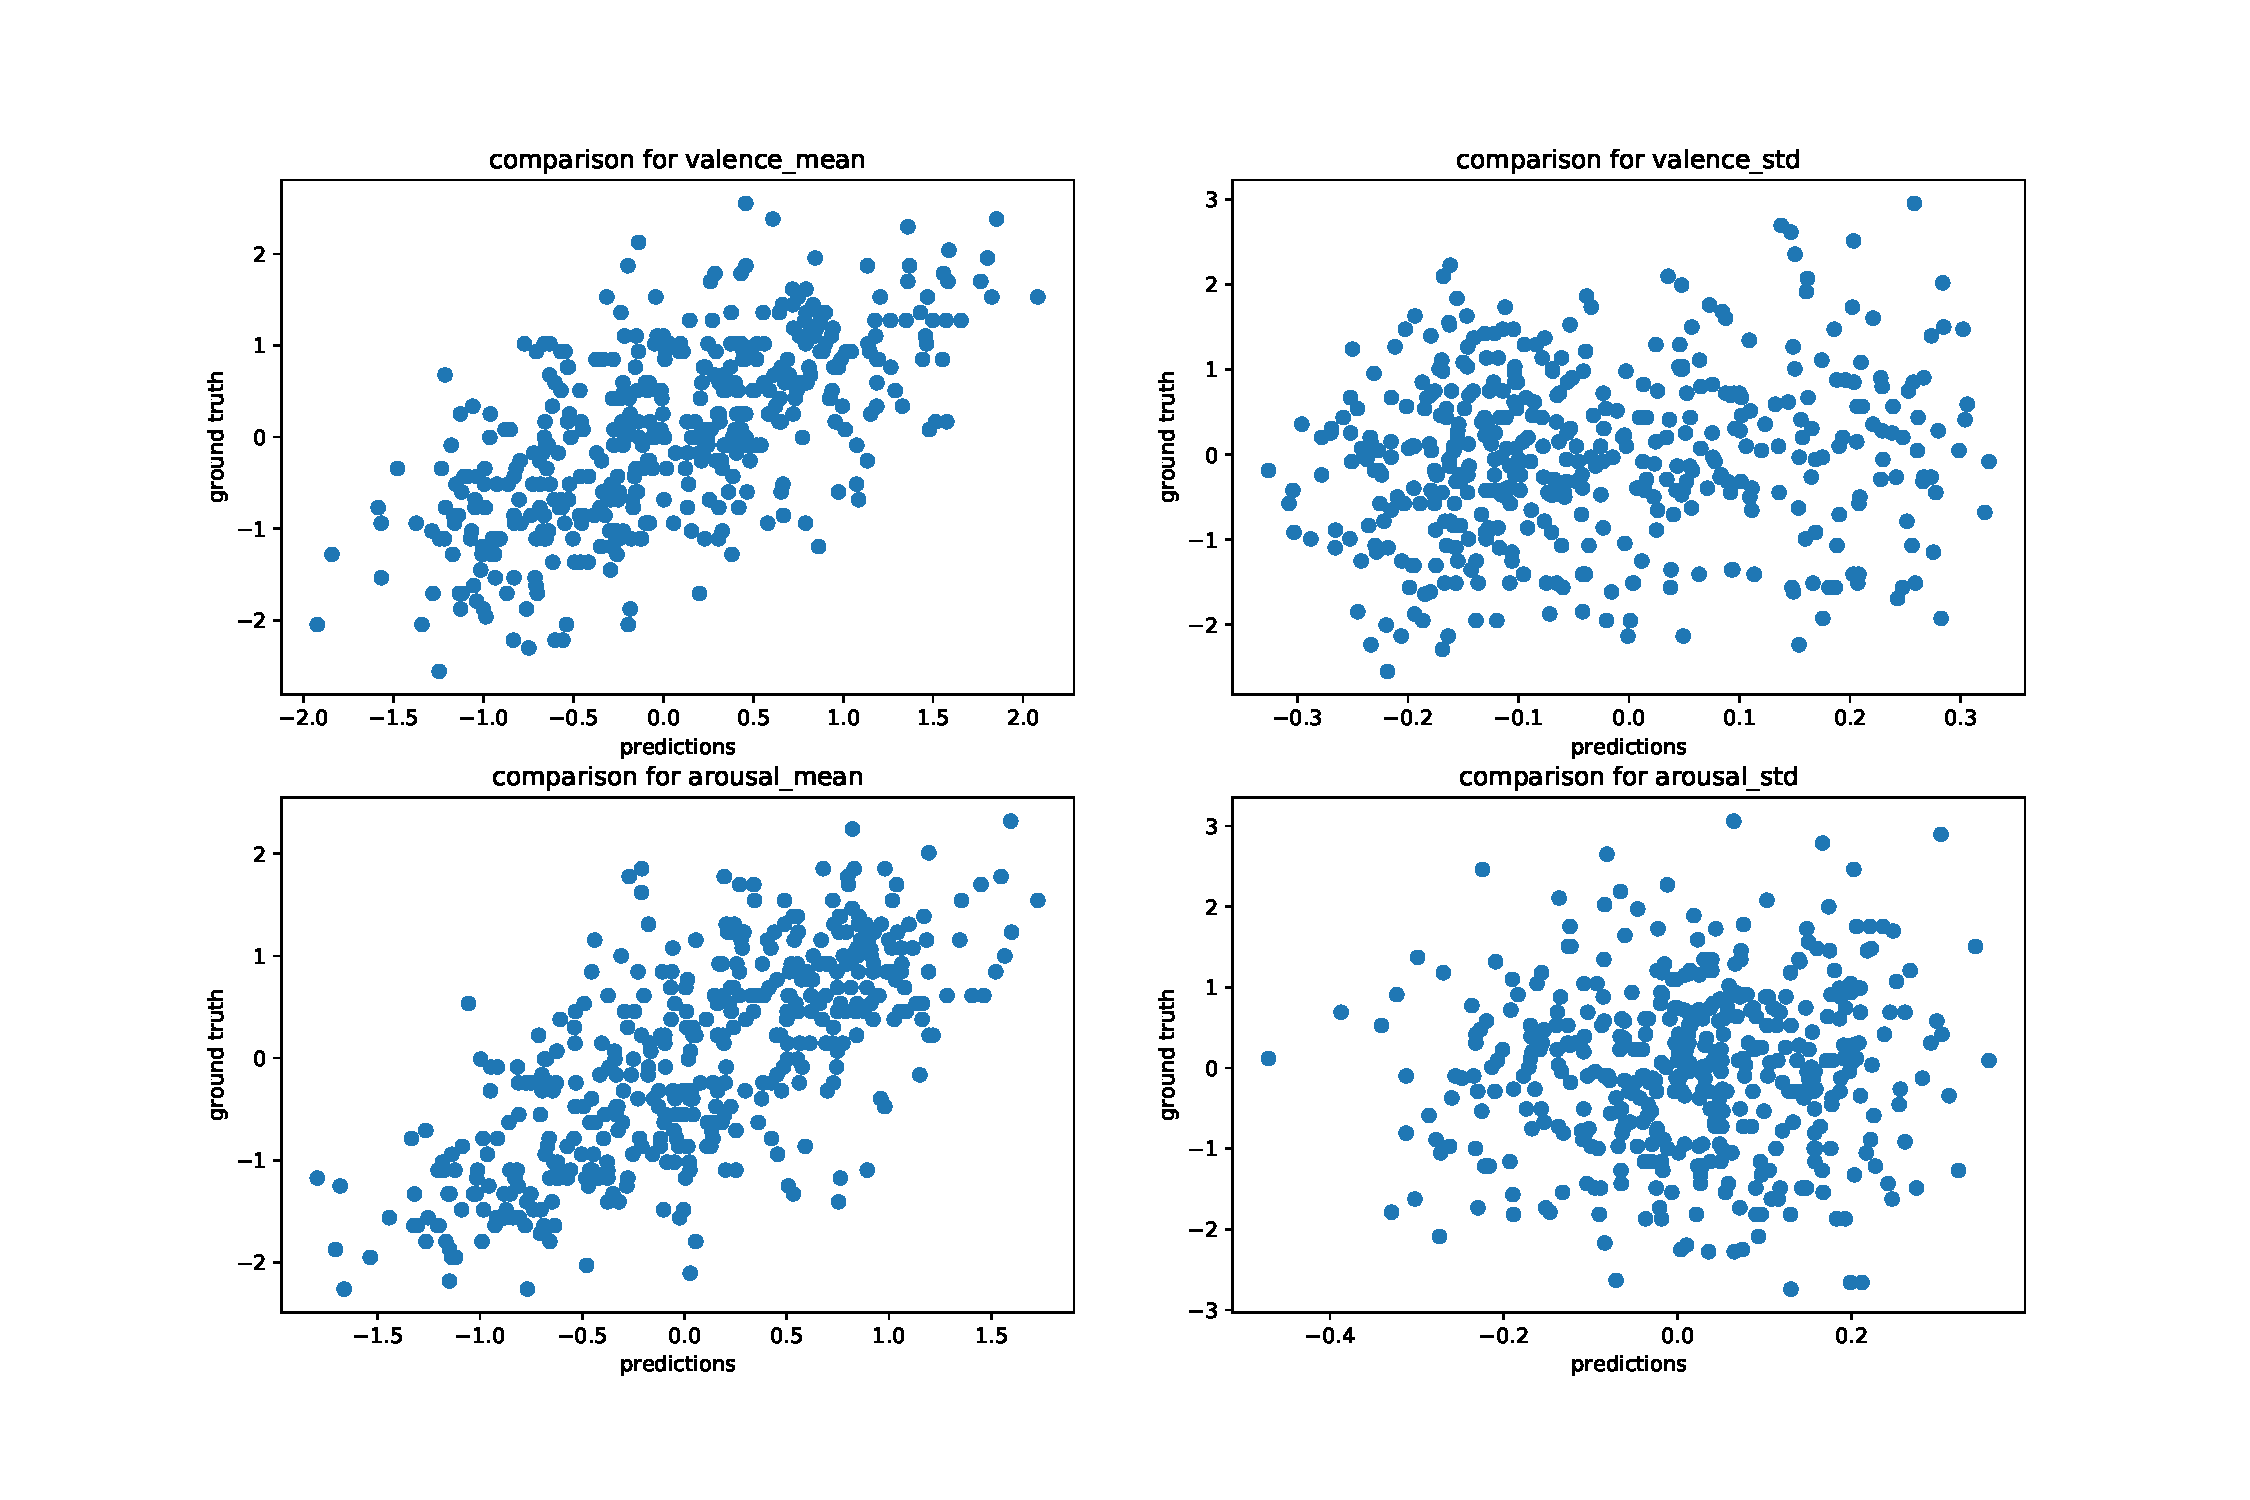
\includegraphics[width=\linewidth]{assets/predictions-scatter.pdf}
	\caption{predictions vs. ground-truth scatter for SVM regression}
	\label{fig:eval-scatter}
\end{figure}


